\begin{figure}
    \centering
    \begin{tabular}{c c c c}
         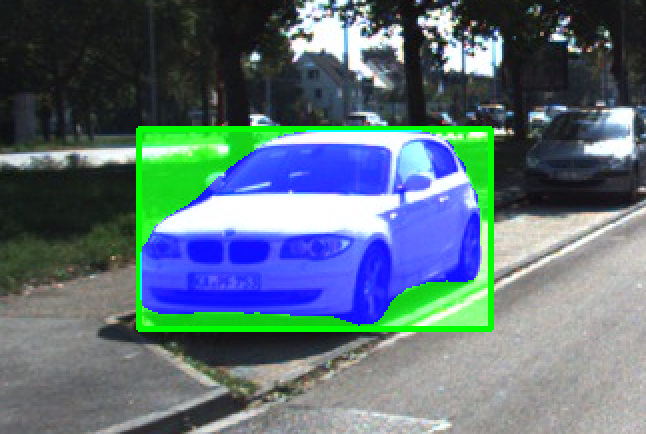
\includegraphics[width=0.25\textwidth]{figures/method/examples/rgb-2.png}
        &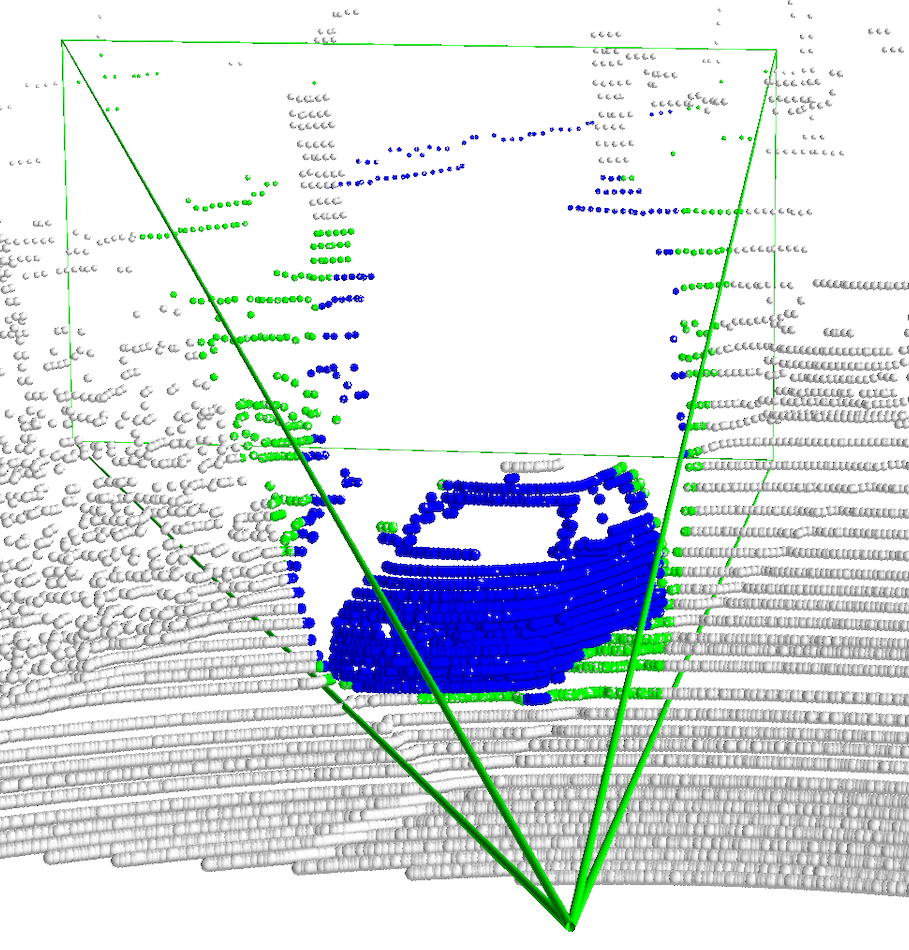
\includegraphics[width=0.2\textwidth]{figures/method/examples/pcd-2.png} &
         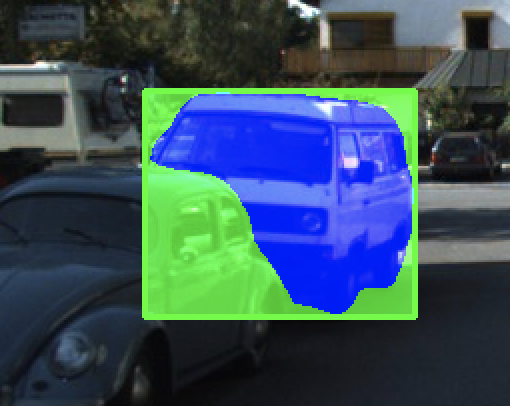
\includegraphics[width=0.2\textwidth]{figures/method/examples/rgb-4.png}
        &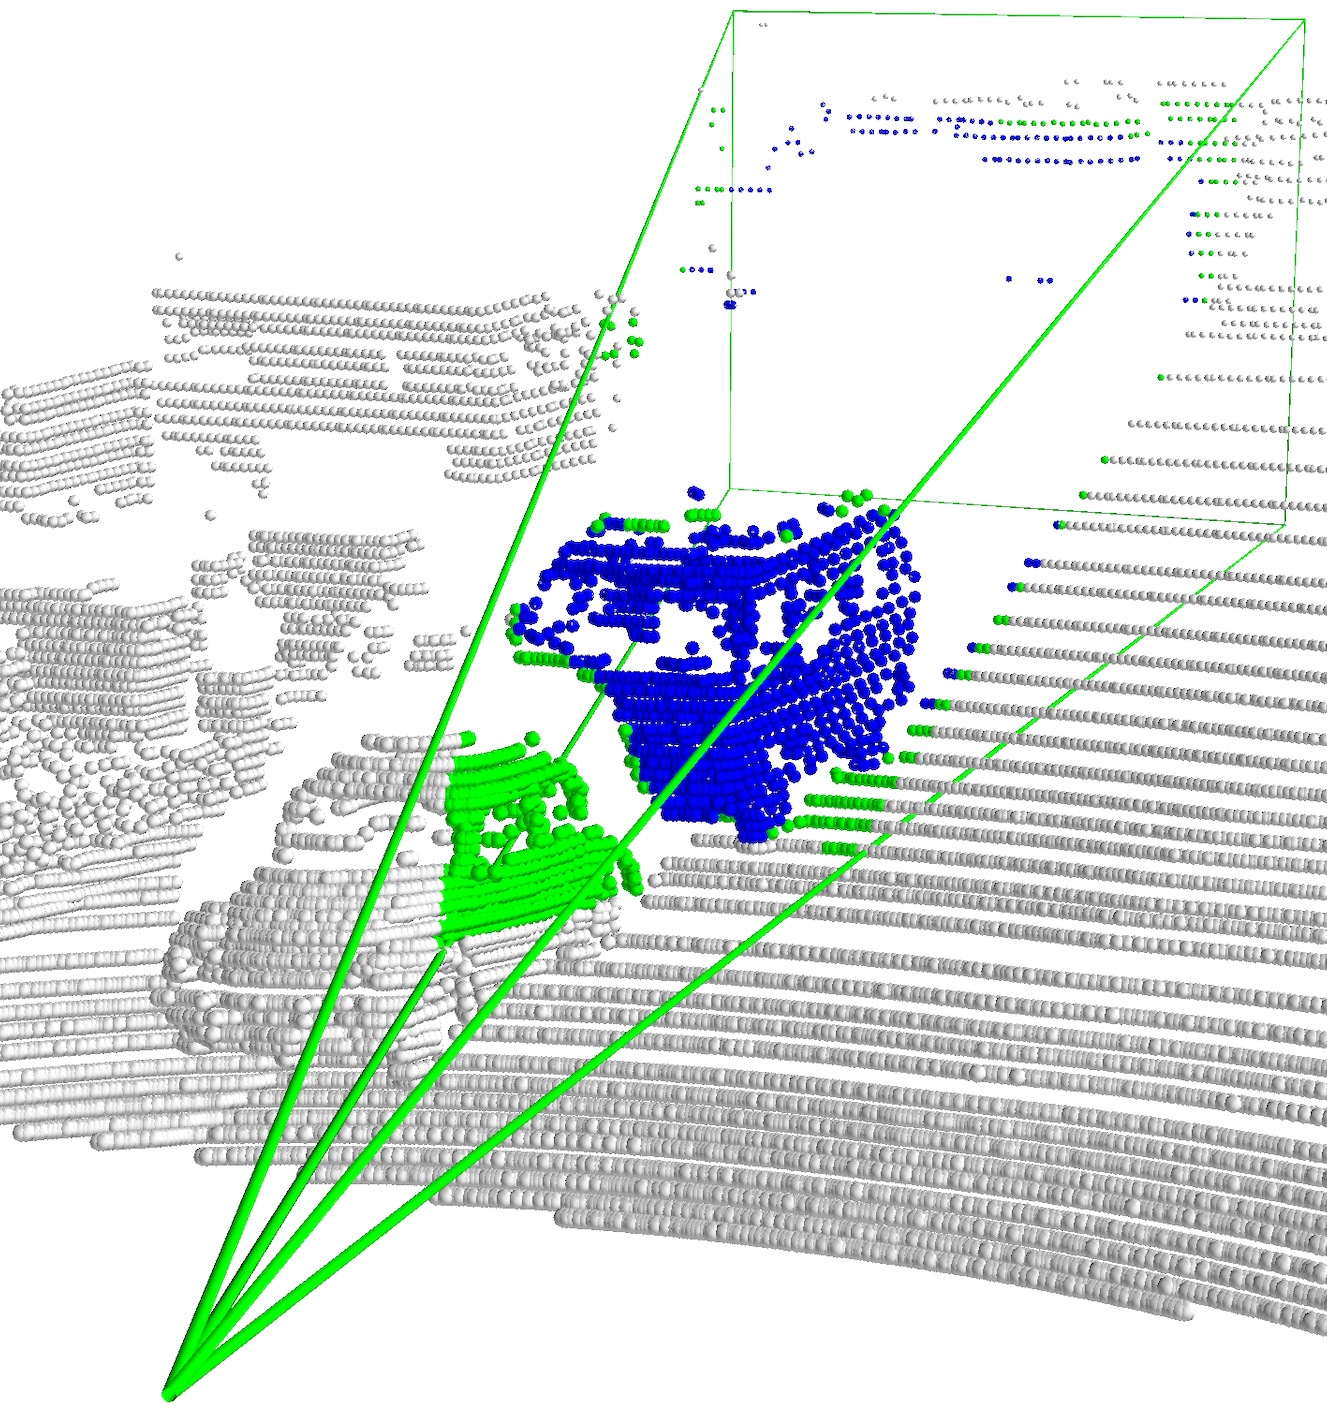
\includegraphics[width=0.2\textwidth]{figures/method/examples/pcd-4.png} \\
    \end{tabular}
    \caption{
    For each pair, left: RGB input image with Mask R-CNN predicted box and highlighted pixels inside the mask.
    Right: LiDAR points in blue represent those inside the 2D mask, green those outside.
    Note that, while the image mask removes many outliers, not all of them ares.}\label{fig:dataset_example}
\end{figure}
